\documentclass{standalone}
\usepackage{tikz}
\usepackage{ctex,siunitx}
\setCJKmainfont{Noto Serif CJK SC}
\usepackage{tkz-euclide}
\usepackage{amsmath}
\usetikzlibrary{patterns, calc,3d}
\usetikzlibrary {decorations.pathmorphing,decorations.pathreplacing,decorations.shapes}
\begin{document}
\small
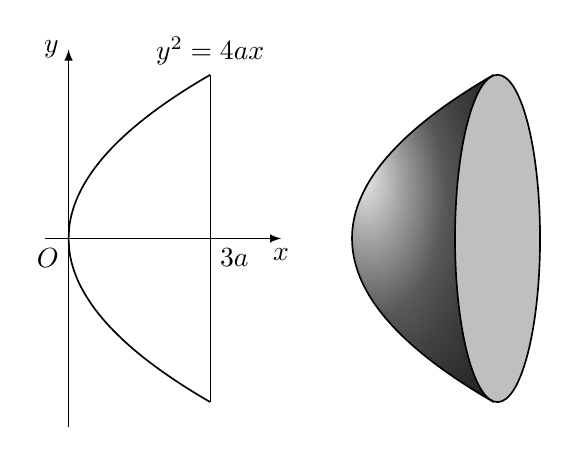
\begin{tikzpicture}[>=latex,scale=0.6]
  \draw[->](-0.5,0)--(4.5,0)node[below]{$x$};
  \draw[->](0,-4)--(0,4)node[left]{$y$};
  \node at (0,0)[below left]{$O$};
  \draw[semithick,domain=0:3,samples=200]plot(\x,{2*sqrt(\x)})node[above]{$y^2=4ax$};
  \draw[semithick,domain=0:3,samples=200]plot(\x,{-2*sqrt(\x)});
  \draw(3,{2*sqrt(3)})--(3,{-2*sqrt(3)})node[midway,below right]{$3a$};
  \begin{scope}[xshift=6cm]
    \draw[semithick,ball color=gray](3,{2*sqrt(3)})..controls(-1,1.1547)and(-1,-1.1547)..(3,{-2*sqrt(3)});
    \draw[semithick,fill=lightgray](3.08,0)ellipse(0.9 and {2*sqrt(3)});
  \end{scope}
\end{tikzpicture}
\end{document}